Manifold learning algorithms, also known as embedding algorithms, map
data from high or infinite-dimensional spaces down
to coordinates in a much lower-dimensional space. In the sciences, one
of the goals of dimension reduction is the discovery of descriptors of
the data generating process. Both linear dimension reduction
algorithms like Principal Component Analysis (PCA) and non-linear algorithms
such as Diffusion Maps \citep{coifman:06} are used in applications from genetics to astronomy to uncover the variables describing
large-scale properties of the interrogated system.

For example, in chemistry, a common objective is to discover so-called
{\em collective coordinates} describing the evolution of molecular
configurations at long time scales, which correspond to
macroscopically interesting transformations of the molecule, and can
explain some of its
properties \citep{clementiOnuchicNymeyer:00,Noe2017-up}.
Figure \ref{fig:molecs} illustrates how manifold learning is used for this purpose. In {\em Molecular Dynamics (MD) simulations}, a molecular configuration is represented by the $3N_a$ vector of spatial locations of the $N_a$ atoms comprising the molecule. A MD simulation produces a sample of molecular configurations; the distribution of this sample describes the molecule's behavior in the given experimental conditions. It has been shown empirically that manifolds  approximate these high-dimensional distributions \citep{Dsilva13-Nonlinear}. 

Figure \ref{fig:toluene-bonds} shows the toluene molecule, consisting of $N_a=15$ atoms, and \ref{fig:tol_circ} shows the mapping of an MD simulated trajectory into $m=2$ dimensions (the embedding coordinates) by a manifold learning algorithm. Visual inspection shows that this configuration space is well-approximated by a one-dimensional manifold parametrized by a geometric quantity, the {\em torsion} $g_1$ of the methyl bond, which is the angle formed by the planes inscribing the first three and last three atoms of the colored lines joining four atoms in Figure \ref{fig:tol_circ}. Thus, $g_1$ is a collective coordinate describing the "slow motions'' of the toluene molecule, filtered out from the faster modes of vibration by the manifold learning algorithm. 
%
\begin{figure}[htb]
\subfloat[][Toluene]{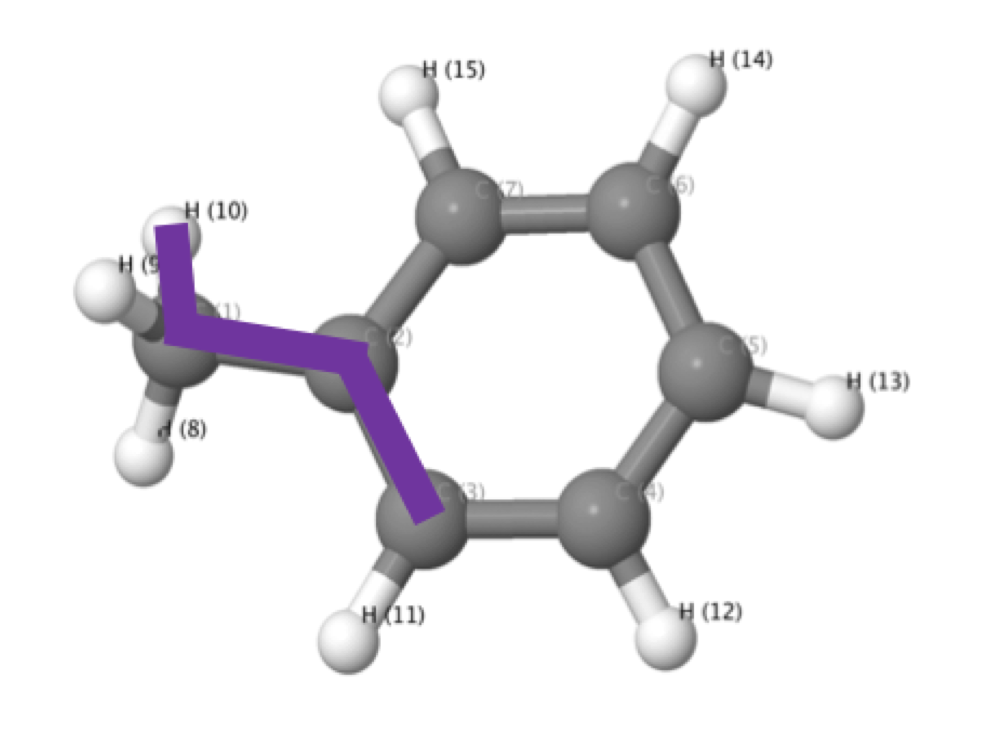
\includegraphics[width=3cm, height=3cm, trim={-.5cm, -.5cm,
-.5cm, -.5cm}, clip]{../Figures/tolbonds}\label{fig:toluene-bonds}}\hfill
\subfloat[][Ethanol]{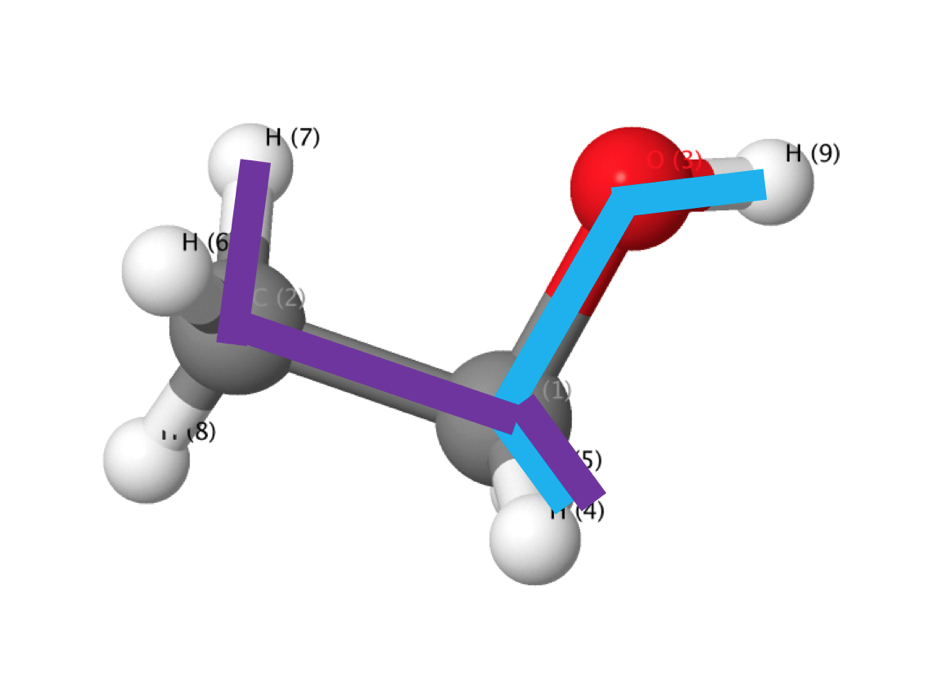
\includegraphics[width=3cm, height=3cm, trim={-1cm, -1cm,
-1cm, -1cm}, clip]{../Figures/ethbonds}\label{fig:ethanol-bonds}}\hfill
\subfloat[][Malonaldehyde]{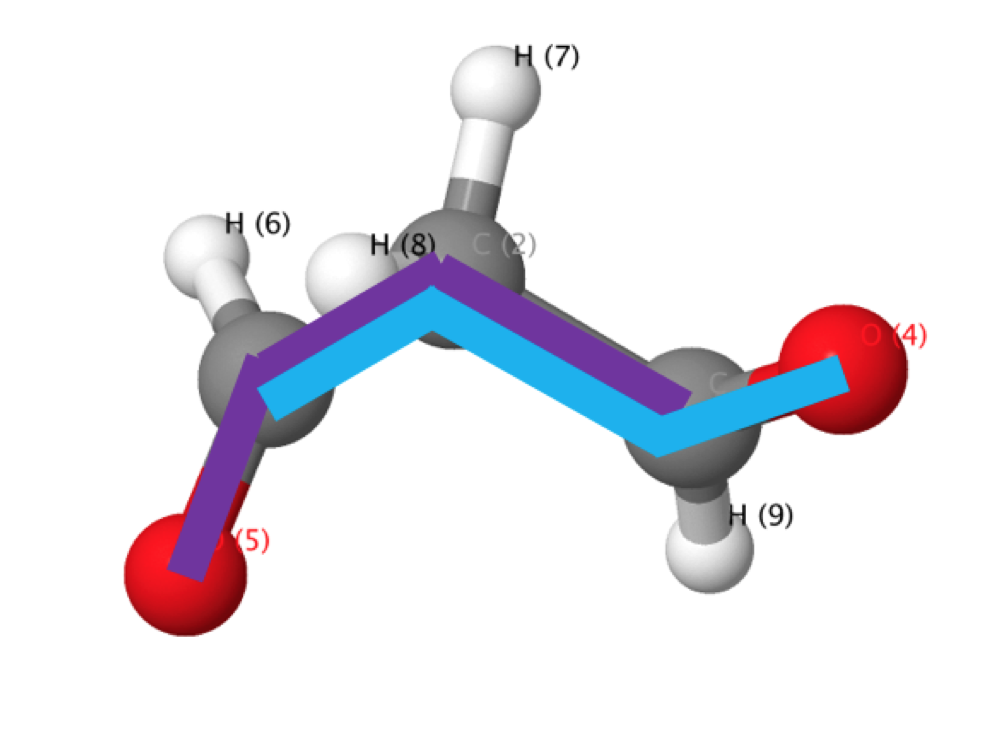
\includegraphics[width=3cm, trim={0, -3cm, 0, 0},
clip]{../Figures/malbonds}\label{fig:mda-bonds}}\hfill \newline
\subfloat[][$g_1$]{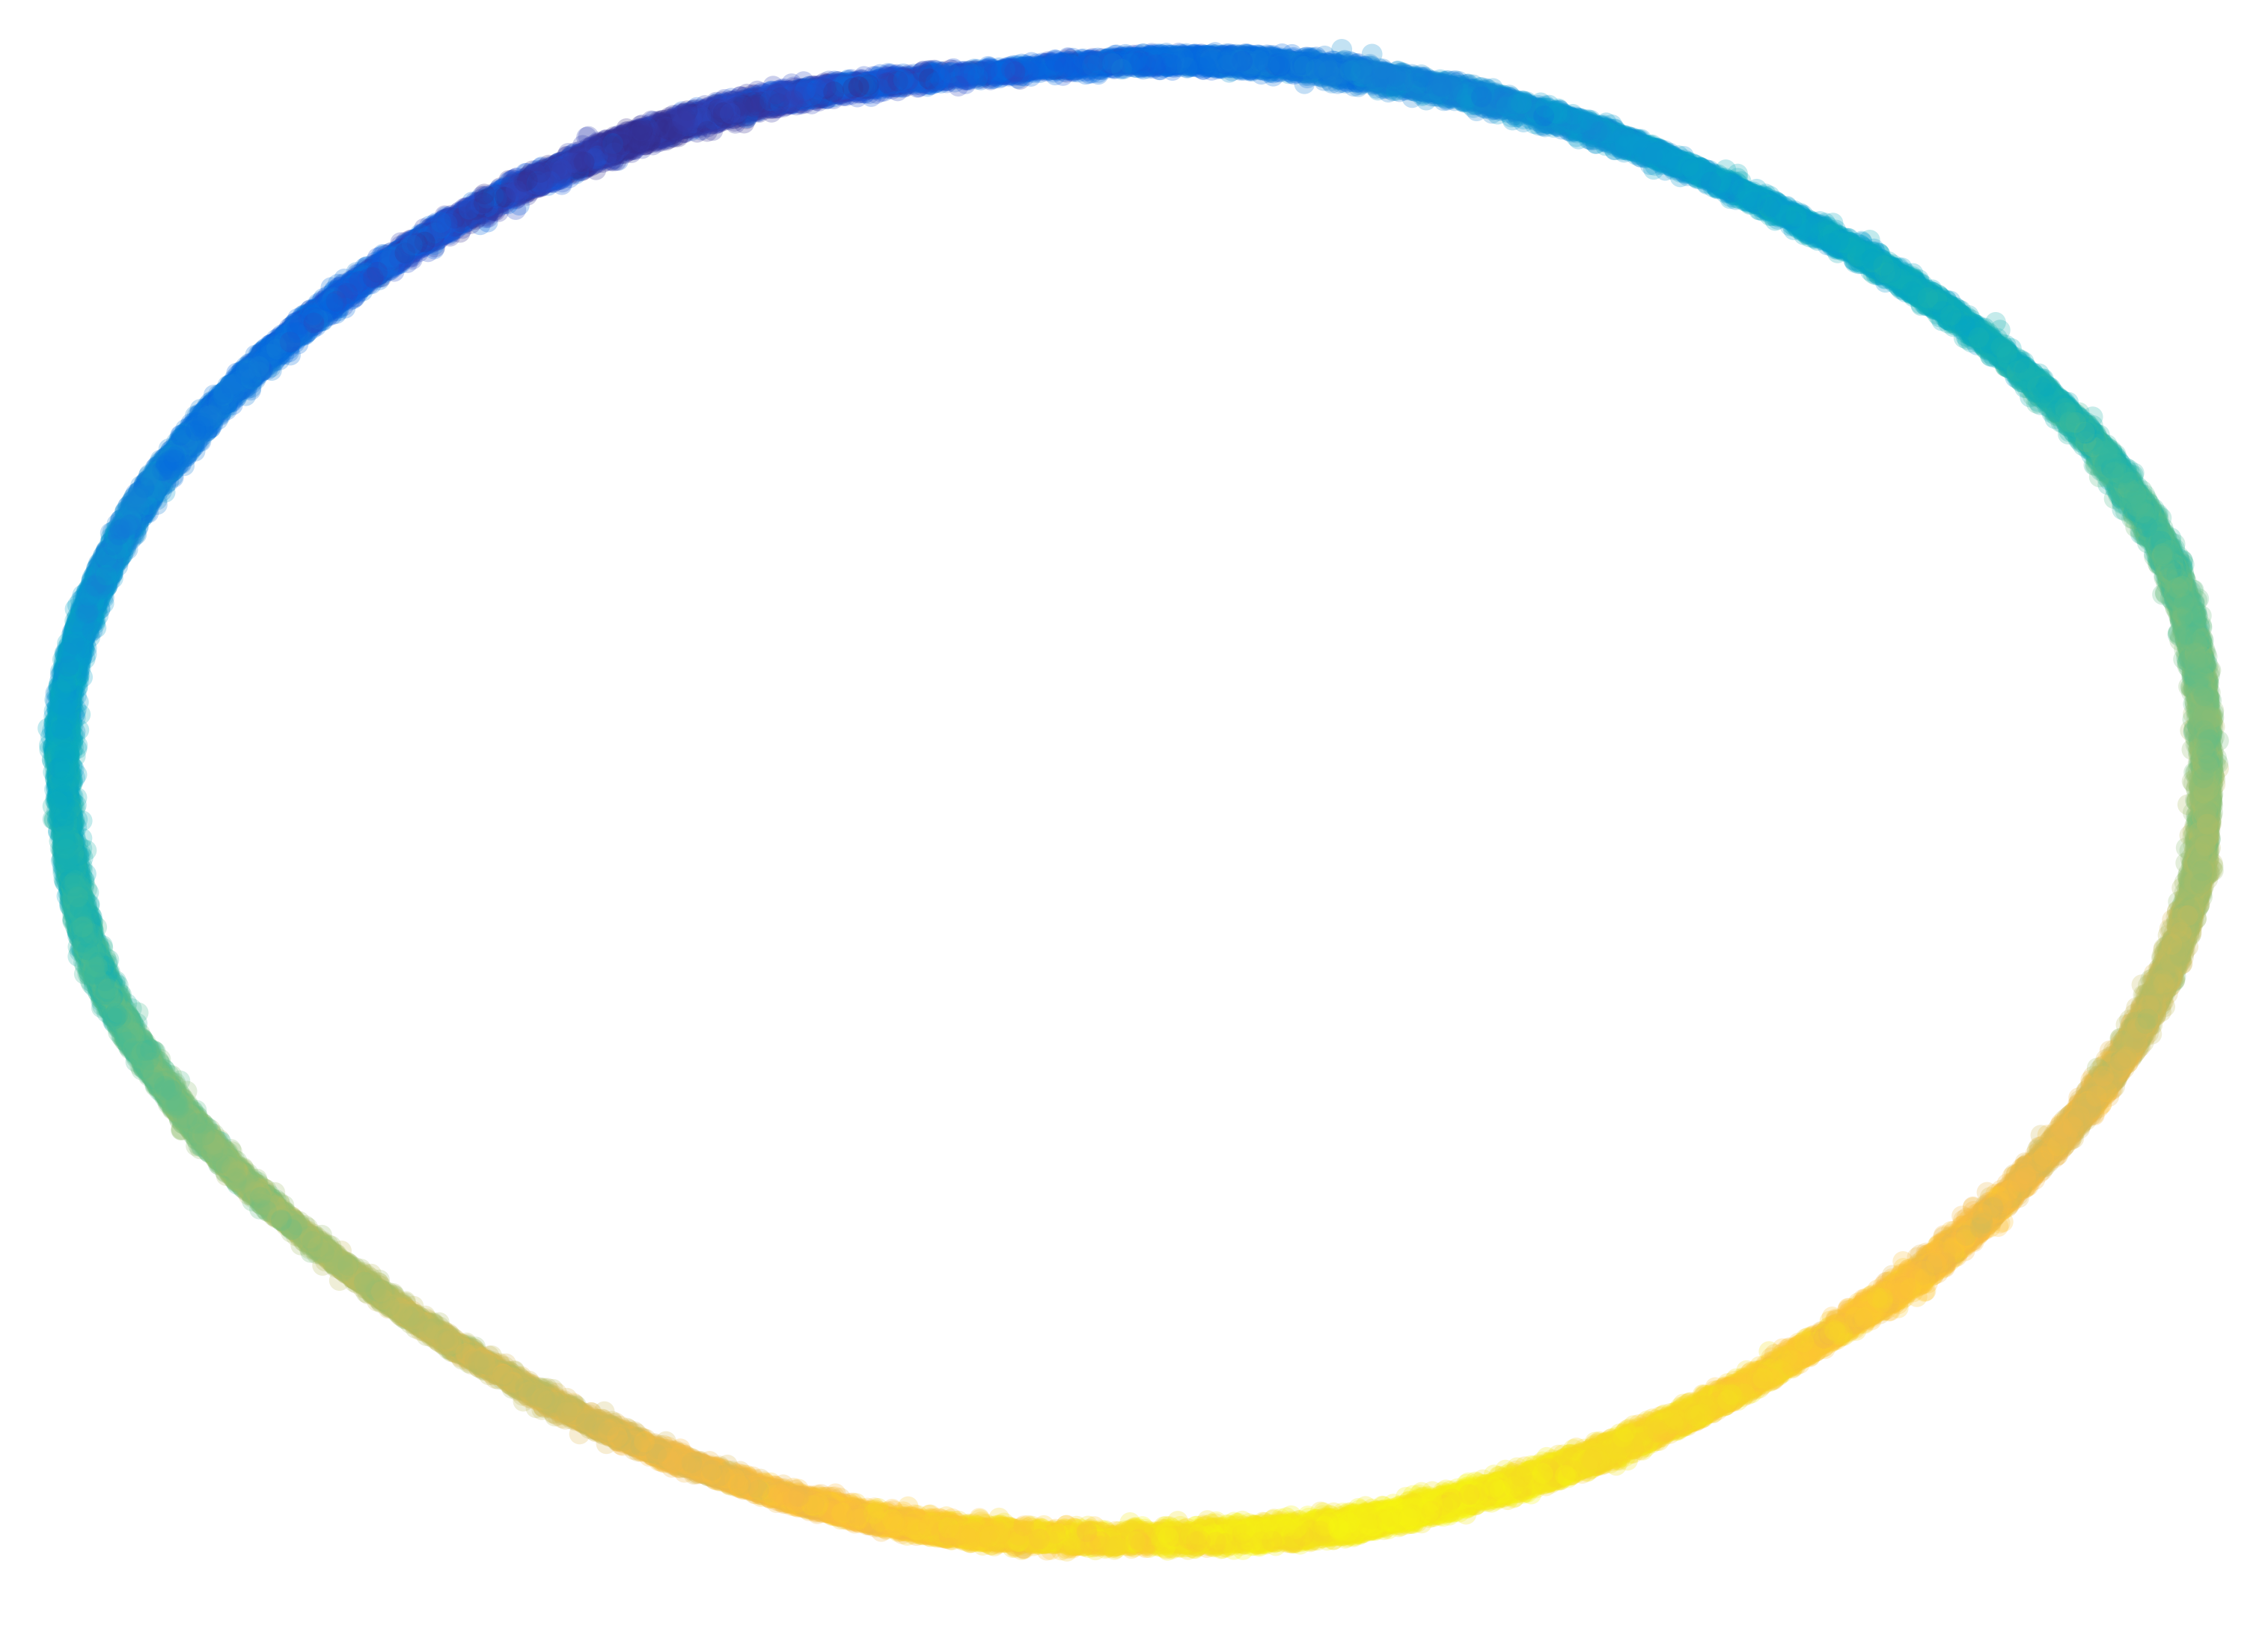
\includegraphics[width=3cm, height=3cm, trim={-1cm, -1cm,
-1cm, -1cm}, clip]{../Figures/toluene-embedding-deformation-torsion.png}\label{fig:tol_circ}}\hfill
\subfloat[][$g_1$]{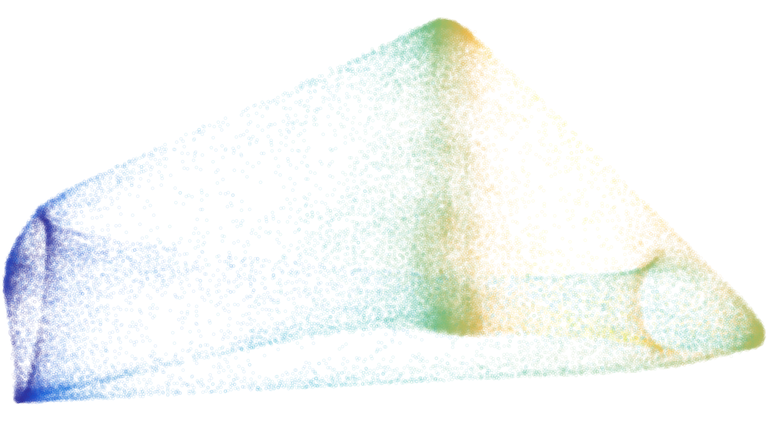
\includegraphics[width=3cm, height=3cm, trim={-1cm, -1cm,
-1cm, -1cm}, clip]{../Figures/ethanoltorsion1.png}\label{fig:eth_tor1}}\hfill
\subfloat[][$g_1$]{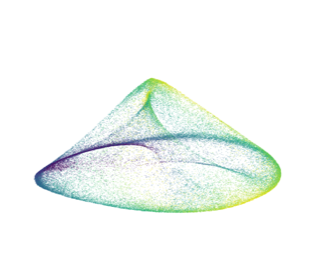
\includegraphics[width=3cm, trim={.5cm, .5cm,
.5cm, .5cm},
clip]{../Figures/malonaldehyde/g1.png}\label{fig:mal_tor1}}\hfill \newline
\subfloat[][Torsion example]{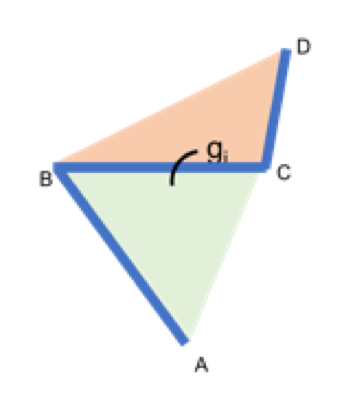
\includegraphics[width=3cm, trim={.5cm, .5cm,
.5cm, .5cm},
clip]{../Figures/torsionexplain.png}\label{fig:tor_explain}}\hfill 
%\hbox to 60.0mm{}
\subfloat[][$g_2$]{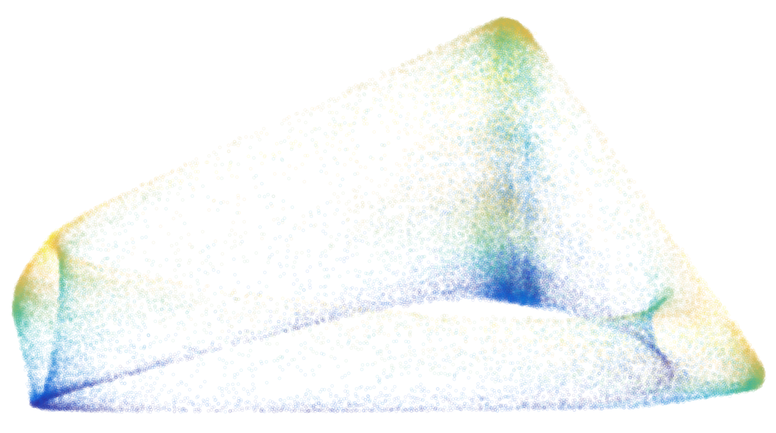
\includegraphics[width=3cm, height=3cm, trim={-1cm, -1cm,
-1cm, -1cm}, clip]{../Figures/ethanoltorsion2.png}\label{fig:eth_tor2}}\hfill
\subfloat[][$g_2$]{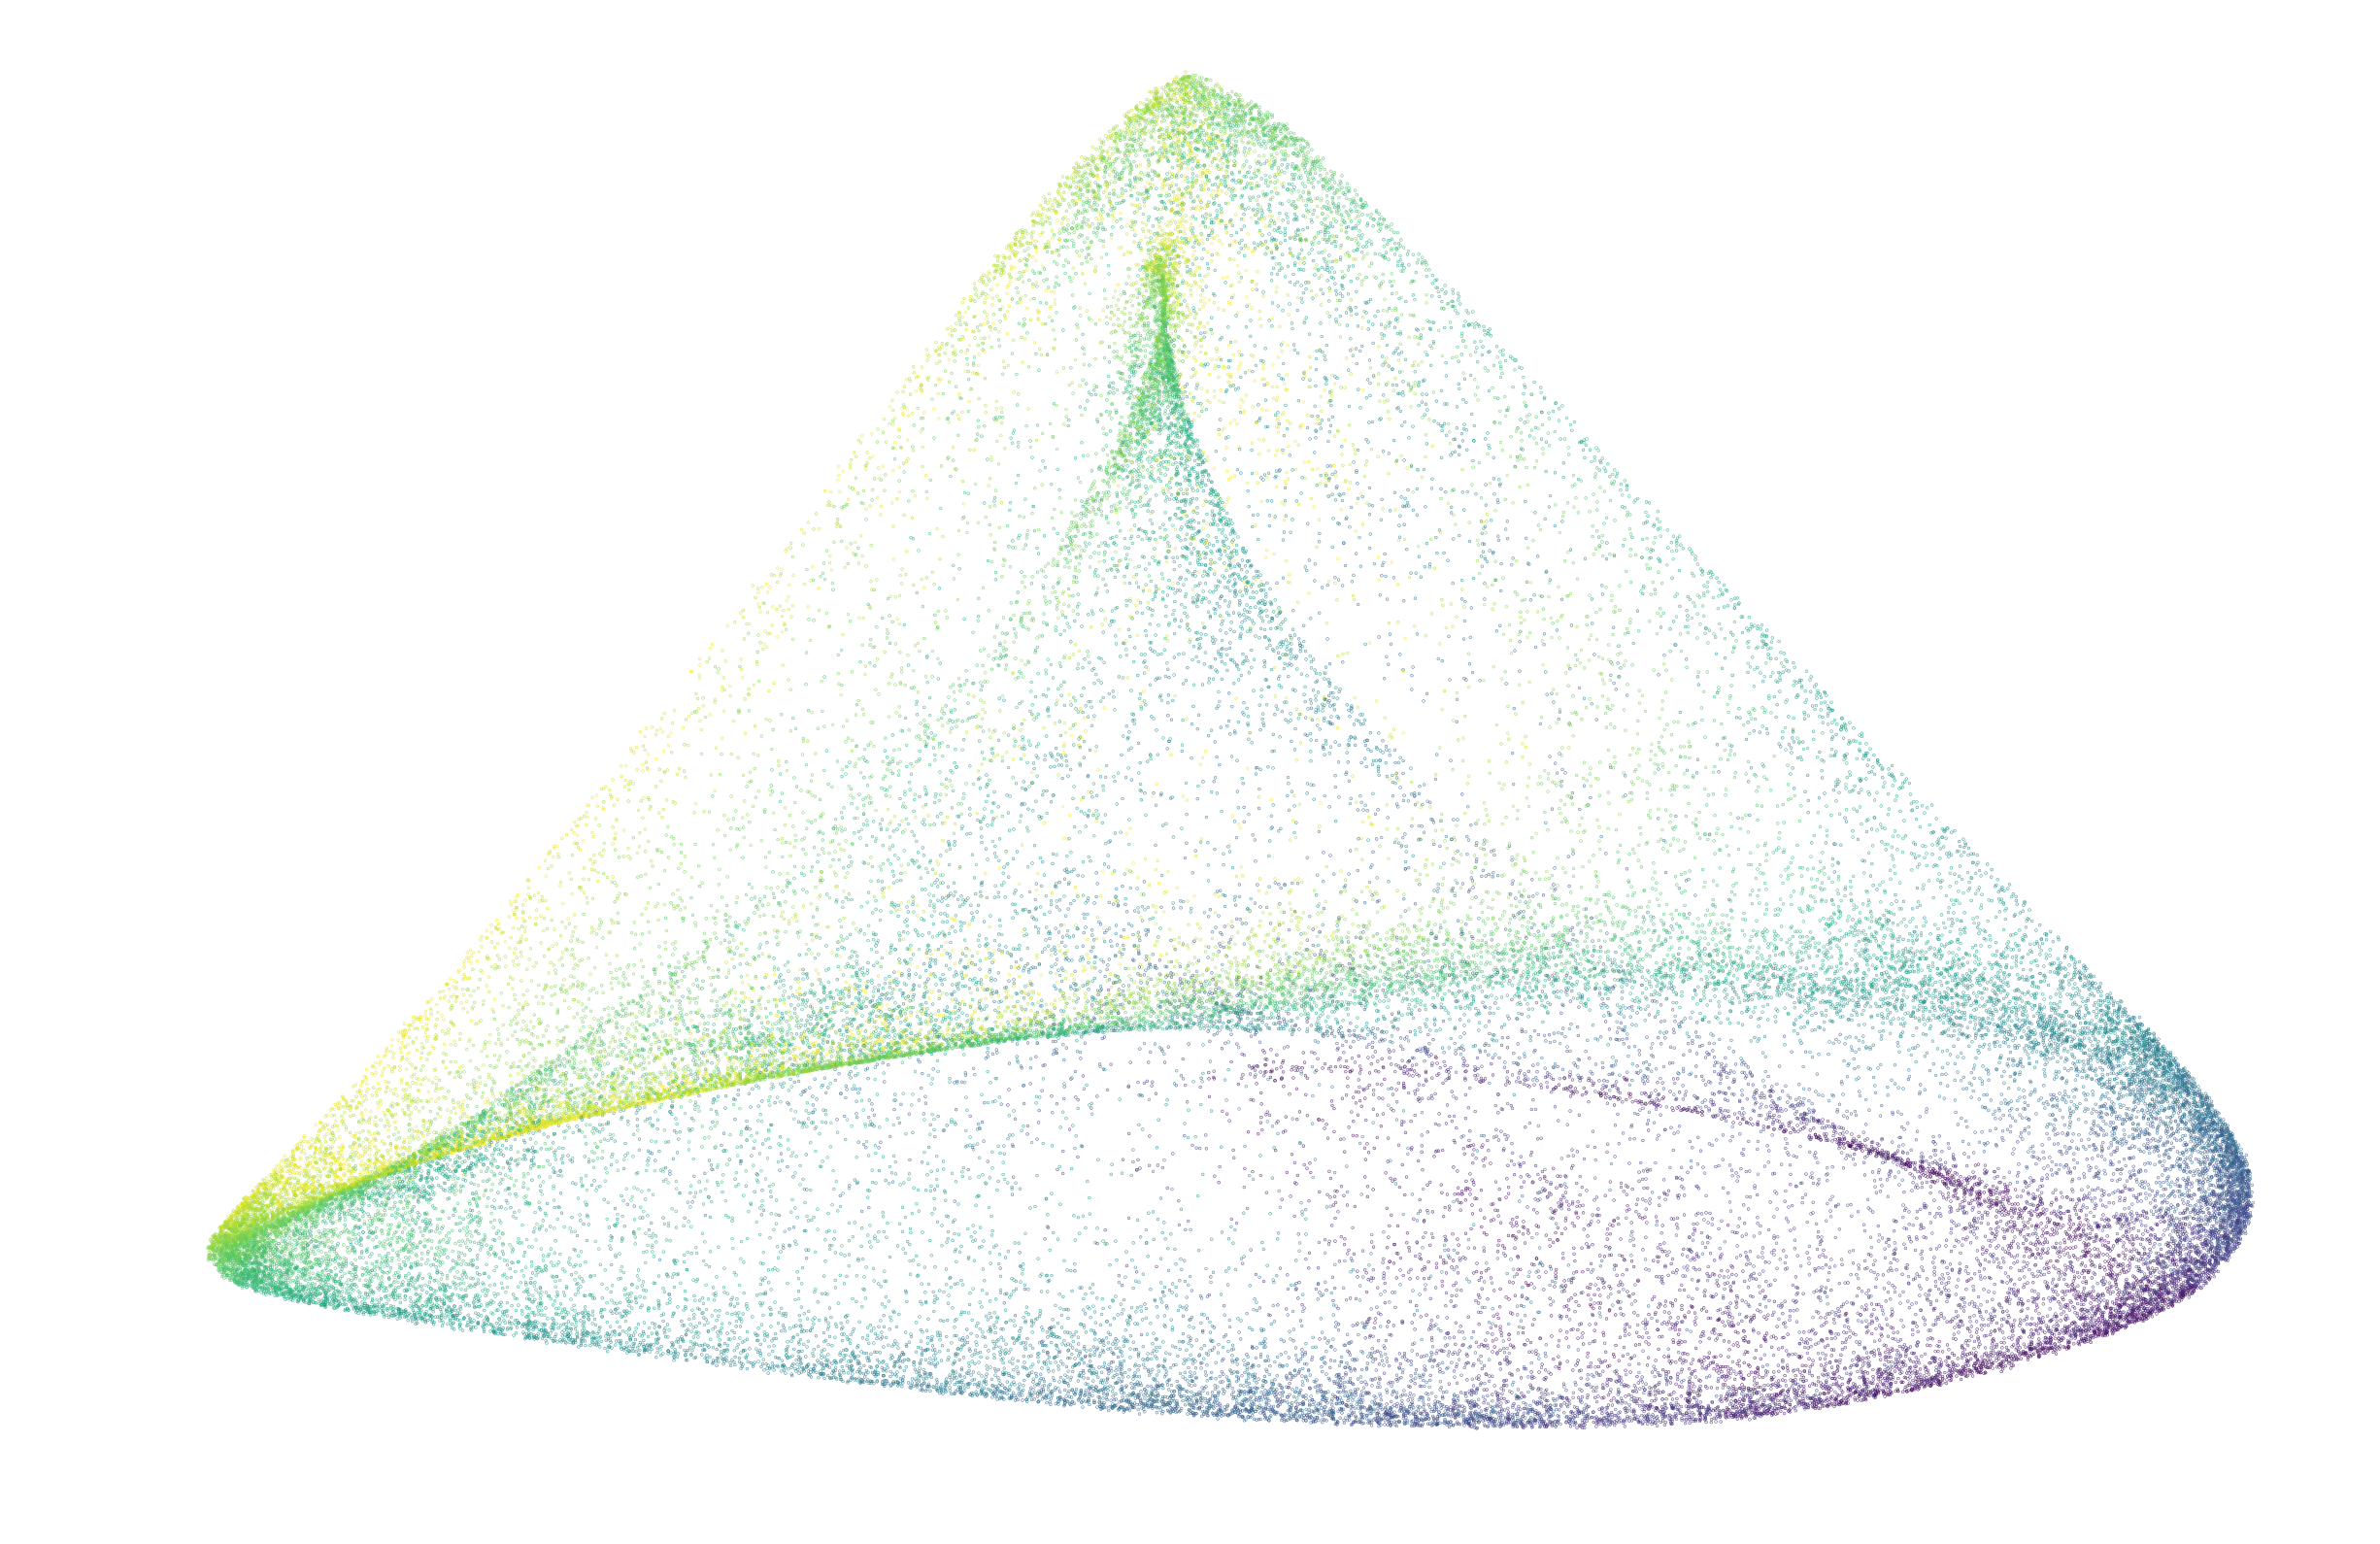
\includegraphics[width=3cm, trim={0, -3cm, 0, 0},
clip]{../Figures/malonaldehyde/April_01_2019_22_23_48/embeddingpic2.png}\label{fig:mal_tor2}}\hfill 
\caption{Collective coordinates with physical meaning in Molecular Dynamics (MD) simulations. \ref{fig:toluene-bonds}-\ref{fig:mda-bonds} Diagrams of the toluene ($C_7 H_8$), ethanol ($C_2H_5OH$), and malonaldehyde ($C_3H_4O_2$) molecules, with the carbon (C) atoms in grey, the oxygen (O) atoms in red, and the hydrogen (H) atoms in white. Bonds defining important torsions $g_j$ are marked in purple and blue  (see Section \ref{sec:exps} for more details). The bond torsion is the angle of the planes inscribing the first three and last three atoms on the line (\ref{fig:tor_explain}).  \ref{fig:tol_circ} Embedding of the configurations of toluene into $m=2$ dimensions, showing a manifold of $d=1$. The color corresponds to the values of the purple torsion $g_1$. \ref{fig:eth_tor1}, \ref{fig:eth_tor2} Embedding of the configurations of the ethanol in $m=3$ dimensions, showing a manifold of dimension $d=2$, respectively colored by the blue and purple torsions in Figure \ref{fig:ethanol-bonds}. \ref{fig:mal_tor1}, \ref{fig:mal_tor2}. Embedding of the configurations of the malonaldehyde in $m=3$ dimensions, showing a manifold of dimension $d=2$, respectively colored by the blue and purple torsions in Figure \ref{fig:mda-bonds}.}
    \label{fig:molecs}
%, as follows: in \ref{fig:toluene-bonds} the purple torsion represents the rotation of the $CH_3$ {\em methyl} group, relative to the $C_6H_5$ {\em benzene} group; in \ref{fig:ethanol-bounds} the purple torsion represents the rotation of the methyl group relative to the middle $CH_2$ group, and the blue torsion the rotation of the $OH$ {\em hydroxyl} group relative to the same $CH_2$ group; in \ref{fig:mda-bonds}, the two torsions respectively represent the rotation of the left and right $CO$ {\em carbonyl} groups relative to the central $CH_2$ group. 
\end{figure}
%

While embedding algorithms are able to uncover the manifold structure of these data, finding the physical meaning of the 1D manifold coordinate in Figure \ref{fig:tol_circ} was done by visual inspection. In general, a trained human expert would scan through many torsions and other functions of the configuration, in order to find ones that can be identified with the abstract coordinates output by a PCA or ML algorithm. Manual inspection of denoised coordinates for features of interest is pervasive in a variety of scientific fields \citep{Chen2016-eq, Herring2018-cq}. The goal of this paper is to put this process on a formal basis and to devise a method for automating this identification, thus removing the time consuming visual inspections from the shoulders of the scientist. We introduce a method to semi-automatically establish relationships of the meaningless abstract coordinates output by an embedding algorithm with functions of the data that are meaningful or interesting in the domain of the problem.

In our paradigm, the scientist inputs a {\em dictionary} $\G$
of functions to be considered as possible collective coordinates. For the examples
in Figure \ref{fig:molecs}, $\G$ could be a set of candidate
torsions. We propose an algorithm that recovers a set of functions
$g_1,\ldots g_s\in\G$, so that $(g_{1:s})$ is a local diffeomorphism
to the output of the embedding algorithm; in other words, so that
$(g_{1:s})$ are collective coordinates for the manifold. To keep the approach as
general as possible, we do not rely on a particular embedding
algorithm, making only the minimal assumption that it produces a
smooth embedding. We also do not assume a parametric relationship
between the embedding and the functions in the dictionary $\G$. Hence,
we only assume that the mapping between the data manifold and the
functions is sufficiently smooth. 

Our method is to compose differentials of functional covariates to
reconstruct the differentials of the manifold embedding coordinates, and is
therefore robust to non-linearity in both the algorithm and the
functional covariates. In other words, by considering differentials,
we map our original non-linear, non-parametric problem to a 
linear sparse regression.

The next section defines the problem formally,
and Section \ref{sec:background} presents the necessary background in manifold
estimation. Section \ref{sec:ouralg} develops our method, \ouralg.  
The relationship to previous work is discussed in
Section \ref{sec:related}. Section \ref{sec:theory} presents theoretical recovery results,  Section \ref{sec:exps} presents experiments, and Section \ref{sec:conc} concludes the paper. The Appendices present details of the functional dictionaries used as well as the adaptions necessary to make our method work in the rotation and translation invariant molecular configuration space.

